\documentclass[11pt,a4paper]{article}

% ==================================================================
% ASR Working Paper - revised technical-review edition
% Compile from the paper/ directory.
% ==================================================================

\usepackage[T1]{fontenc}
\usepackage[utf8]{inputenc}
\usepackage{amsmath,amsthm}
\usepackage{newtxtext,newtxmath}
\usepackage[margin=1in]{geometry}
\usepackage{graphicx}
\usepackage{booktabs}
\usepackage{array}
\usepackage{caption}
\usepackage[round,authoryear]{natbib}
\usepackage[hidelinks]{hyperref}
\usepackage{xurl}
\usepackage{enumitem}
\usepackage{fancyhdr}
\usepackage{setspace}
\usepackage{microtype}

\onehalfspacing
\setlength{\parindent}{15pt}
\setlength{\parskip}{0pt}
\setlength{\headheight}{14pt}
\emergencystretch=1em

% Compile from paper/: figure files are stored in ../figures/.
\graphicspath{{../figures/}}

\newtheorem{proposition}{Proposition}
\newtheorem{remark}{Remark}

\DeclareMathOperator{\Var}{Var}
\newcommand{\Prob}{\mathbb{P}}
\newcommand{\E}{\mathbb{E}}
\newcommand{\dd}{\,\mathrm{d}}

% ==================================================================
% Publication and software metadata
% ==================================================================
\newcommand{\PaperVersion}{v3}
\newcommand{\PaperDate}{16 July 2026}
\newcommand{\ConceptDOI}{10.5281/zenodo.21385498}
\newcommand{\SoftwareVersion}{1.1.0}
\newcommand{\ReviewedCommit}{0b62582a44be2d401db4e0d68e2ed1fa72d56bc4}

\hypersetup{
  pdftitle={Bachelier's Theory of Speculation Revisited: A Reproducible Reconstruction of the Origins of Quantitative Finance},
  pdfauthor={Alpha Kabinet TOURE},
  pdfsubject={A technically reviewed and reproducible reconstruction of the Bachelier arithmetic Brownian motion and normal option-pricing model},
  pdfkeywords={Louis Bachelier, Bachelier model, arithmetic Brownian motion, normal option pricing, quantitative finance, Monte Carlo simulation, reproducible research, open science}
}

\pagestyle{fancy}
\fancyhf{}
\fancyhead[C]{\small\itshape Bachelier's Theory of Speculation Revisited}
\fancyfoot[C]{\small\thepage}
\renewcommand{\headrulewidth}{0.4pt}
\renewcommand{\footrulewidth}{0pt}

\title{\textbf{Bachelier's Theory of Speculation Revisited:\\
A Reproducible Reconstruction of the Origins\\
of Quantitative Finance}}

\author{
Alpha Kabinet TOURE\\
\normalsize Alpha Stochastic Research
\thanks{%
Alpha Stochastic Research. Correspondence: \texttt{research@asr-lab.online}.\\
Concept DOI: \href{https://doi.org/\ConceptDOI}{\ConceptDOI}.\\
Replication code, figures, tests, and documentation:
\url{https://github.com/Alpha-Stochastic-Research/asr-theory-of-speculation}.%
}
}

\date{\PaperDate\\[3pt]
\small ASR Working Paper, Version \PaperVersion\ -- Technical-review revision}

\begin{document}

\maketitle
\thispagestyle{empty}

\begin{abstract}
\noindent
Louis Bachelier's 1900 doctoral thesis, \emph{Th\'eorie de la Sp\'eculation}, is one of the earliest mathematical foundations of modern quantitative finance. This paper provides a modern and computationally reproducible reconstruction of selected mathematical elements of Bachelier's theory. We formulate the arithmetic Brownian motion model in contemporary notation, establish its martingale property using conditional expectation, derive its variance-scaling relation, and present the normal European call-pricing formula in an explicit forward-measure and discounting framework. We then numerically corroborate the analytical results through fixed-seed Python simulations, Monte Carlo estimation, automated tests, and open-source research materials. A local comparison with Black--Scholes distinguishes normal absolute-price dynamics from lognormal proportional-price dynamics and quantifies their pricing difference under a low-relative-volatility calibration. The contribution is not a new option-pricing theory, but a transparent bridge between Bachelier's historical work, modern mathematical finance, and reproducible computational practice.

\vspace{6pt}
\noindent\textbf{Keywords:} Bachelier; Theory of Speculation; Arithmetic Brownian Motion; Normal Model; Option Pricing; Quantitative Finance; Monte Carlo Simulation; Reproducible Research; Open Science

\vspace{4pt}
\noindent\textbf{JEL Classification:} C15, C63, G12, G13, B26
\end{abstract}

\newpage
\setcounter{page}{1}

% ==================================================================
\section{Introduction}
% ==================================================================

The history of quantitative finance is often narrated through modern portfolio theory, the Black--Scholes--Merton option-pricing framework, and the rise of computational methods. Yet one of the earliest mathematical treatments of speculation predates these developments by several decades. In 1900, Louis Bachelier submitted his doctoral thesis, \emph{Th\'eorie de la Sp\'eculation}, in which he proposed a probabilistic approach to market fluctuations and derived relations for option-like contracts \citep{bachelier1900}.

Bachelier's work is remarkable for at least three reasons. First, it introduced probabilistic reasoning into the study of market prices before financial economics possessed its modern mathematical vocabulary. Second, it anticipated ideas later associated with diffusion processes, derivative valuation, and stochastic modelling. Third, it treated contingent financial contracts as payoff functions whose values could be studied through probability laws.

This paper revisits Bachelier's theory from a modern reproducibility perspective. Rather than treating the 1900 thesis only as a historical document, we reconstruct a selected mathematical core and implement it as an open-source computational research object. The objective is to make the model transparent, executable, testable, and educational for students, researchers, and practitioners.

The paper makes four contributions. First, it formulates arithmetic Brownian motion in contemporary notation and gives a complete conditional-expectation proof of the martingale property. Second, it presents the normal European call formula in a financially explicit pricing framework using a forward price, a forward measure, and a discount factor. Third, it numerically corroborates the analytical relations through fixed-seed Monte Carlo experiments and uncertainty reporting. Fourth, it distinguishes the Bachelier and Black--Scholes architectures and quantifies their local pricing difference.

The remainder of the paper is organized as follows. Section~2 reviews the relevant historical and technical literature. Section~3 defines the historical source and scope of the reconstruction. Section~4 presents arithmetic Brownian motion. Section~5 derives the normal call formula. Section~6 describes the computational methodology. Section~7 reports numerical results. Section~8 compares the normal and lognormal models. Sections~9 and~10 discuss interpretation and limitations. Section~11 presents the reproducibility framework, and Section~12 concludes.

% ==================================================================
\section{Literature Review}
% ==================================================================

Bachelier's \emph{Th\'eorie de la Sp\'eculation} is recognized as one of the earliest mathematical treatments of financial markets \citep{bachelier1900}. Its later dissemination in English was aided by its inclusion in \citet{cootner1964} and by subsequent translations and commentaries \citep{bachelier1964,davisetheridge2006}. Historical scholarship has also clarified Bachelier's scientific context, career, reception, and influence on probability and mathematical finance \citep{courtault2000}.

The probabilistic view of price fluctuations developed further in the mid-twentieth century. \citet{osborne1959} examined Brownian motion in stock markets, while \citet{mandelbrot1963} challenged Gaussian assumptions by documenting large variations and heavy-tailed behaviour in speculative prices. These developments illustrate both the historical importance of Gaussian models and their empirical limitations.

Modern option-pricing theory is usually associated with \citet{blackscholes1973} and \citet{merton1973}, who developed a no-arbitrage framework based on geometric Brownian motion and dynamic replication. Earlier, \citet{samuelson1965} connected stochastic modelling with rational warrant valuation. The Black--Scholes--Merton model differs from the simple Bachelier specification in several fundamental respects: prices are lognormal and positive, pricing is explicitly linked to no-arbitrage and replication, and discounting is incorporated within a risk-neutral framework.

Standard references such as \citet{feller1968}, \citet{karatzas1998}, and \citet{shreve2004} provide the mathematical background for Brownian motion, martingales, stochastic calculus, and measure-based pricing. From a financial-engineering perspective, \citet{hull2018} presents derivative-pricing practice, while \citet{bjork2009} gives a rigorous treatment of arbitrage pricing in continuous time.

Bachelier-style normal models remain relevant in modern finance, particularly in interest-rate markets and settings where absolute changes are more natural than proportional returns. Normal volatility also appears in the SABR literature and related volatility-smile approximations \citep{hagan2002}.

The contribution of this paper is therefore methodological and pedagogical rather than theoretical novelty: it provides a self-contained reconstruction using modern notation, explicit pricing assumptions, open-source Python code, numerical uncertainty, automated testing, and archived research metadata.

% ==================================================================
\section{Historical Source and Scope of Reconstruction}
% ==================================================================

The primary historical source is Bachelier's 1900 thesis, \emph{Th\'eorie de la Sp\'eculation}, published in the \emph{Annales Scientifiques de l'\'Ecole Normale Sup\'erieure} \citep{bachelier1900}. The original work combines institutional descriptions of the Paris market with mathematical analysis of speculation, forward transactions, premiums, and probability laws.

This paper does not reproduce every institutional detail of the thesis. Many conventions discussed by Bachelier were specific to the late-nineteenth-century Paris market. Instead, the reconstruction focuses on the mathematical elements that remain central to quantitative finance:

\begin{enumerate}[label=(\roman*), leftmargin=2.2em]
\item the representation of price changes through a probability law;
\item the modern arithmetic-Brownian-motion interpretation;
\item the martingale intuition associated with the absence of directional bias;
\item linear variance growth and square-root-of-time standard deviation;
\item the valuation of option-like payoffs under a normal law.
\end{enumerate}

The reconstruction is mathematical and computational rather than archival. Modern terms such as Brownian motion, filtration, martingale, forward measure, risk-neutral valuation, and Monte Carlo simulation are used to express and evaluate the model in contemporary language; they are not presented as Bachelier's original vocabulary.

\begin{remark}
The paper deliberately distinguishes three layers: Bachelier's historical contribution, its modern probabilistic interpretation, and a contemporary no-arbitrage pricing formulation. This separation avoids attributing later terminology or measure-theoretic arguments directly to the 1900 text.
\end{remark}

% ==================================================================
\section{The Arithmetic Brownian Motion Model}
% ==================================================================

\subsection{Model Specification}

Let \((\Omega,\mathcal{F},(\mathcal{F}_t)_{t\geq0},\Prob)\) be a filtered probability space supporting a standard Brownian motion \((W_t)_{t\geq0}\). Let \(P_t\) denote an illustrative price-level process. The driftless arithmetic Brownian motion model is

\begin{equation}
P_t=P_0+\sigma W_t,
\label{eq:bachelier-process}
\end{equation}

where \(P_0\in\mathbb{R}\) is deterministic and \(\sigma>0\) is an arithmetic volatility measured in price units per square root of time. Equivalently,

\begin{equation}
\dd P_t=\sigma\,\dd W_t.
\label{eq:bachelier-sde}
\end{equation}

Unlike geometric Brownian motion, this specification models absolute price changes rather than proportional returns. For every \(t\geq0\),

\begin{equation}
P_t\sim\mathcal{N}(P_0,\sigma^2t).
\label{eq:normal-price-distribution}
\end{equation}

\subsection{Martingale Property}

\begin{proposition}[Martingale Property]
The process \((P_t)_{t\geq0}\) defined by equation~\eqref{eq:bachelier-process} is an \((\mathcal{F}_t)\)-martingale.
\end{proposition}

\begin{proof}
For \(0\leq s\leq t\),
\[
P_t=P_s+\sigma(W_t-W_s).
\]
The Brownian increment \(W_t-W_s\) is independent of \(\mathcal{F}_s\), integrable, and has zero mean. Therefore,
\[
\E[P_t\mid\mathcal{F}_s]
=P_s+\sigma\E[W_t-W_s\mid\mathcal{F}_s]
=P_s.
\]
Hence \((P_t)_{t\geq0}\) is a martingale. In particular, \(\E[P_t]=P_0\).
\end{proof}

The martingale property does not imply constant realized prices. It states that, conditional on current information and under the chosen measure, the model contains no predictable directional bias.

\subsection{Variance Scaling}

\begin{proposition}[Linear Variance Growth]
Under equation~\eqref{eq:bachelier-process},
\[
\Var(P_t)=\sigma^2t.
\]
\end{proposition}

\begin{proof}
Because \(P_0\) is deterministic and \(\Var(W_t)=t\),
\[
\Var(P_t)=\Var(\sigma W_t)=\sigma^2\Var(W_t)=\sigma^2t.
\]
\end{proof}

Consequently,

\begin{equation}
\sqrt{\Var(P_t)}=\sigma\sqrt{t}.
\label{eq:sqrt-time-volatility}
\end{equation}

The square-root-of-time relation follows exactly under independent Gaussian increments. Its empirical use outside this model requires caution because volatility, dependence, jumps, and market regimes may vary through time.

% ==================================================================
\section{Normal European Call Pricing}
% ==================================================================

\subsection{Pricing Framework}

A probability distribution alone does not determine an arbitrage-free option price. For pricing purposes, we therefore formulate the normal model for a forward price under the corresponding forward measure.

Let \(F_t\) be the time-\(t\) forward price for delivery at maturity \(T\), let \(D(t,T)\) be the discount factor, and let \(\Prob^T\) denote the \(T\)-forward measure. Assume that, for \(t\leq u\leq T\),

\begin{equation}
\dd F_u=\sigma_N\,\dd W_u^T,
\label{eq:forward-normal-dynamics}
\end{equation}

where \(\sigma_N>0\) is the normal or arithmetic volatility and \(W^T\) is a Brownian motion under \(\Prob^T\). Then \(F_u\) is a \(\Prob^T\)-martingale and

\begin{equation}
F_T=F_t+\sigma_N\sqrt{\tau}\,Z,
\qquad \tau=T-t,
\qquad Z\sim\mathcal{N}(0,1).
\label{eq:forward-terminal-law}
\end{equation}

The time-\(t\) value of a European call with strike \(K\) is

\begin{equation}
C_t=D(t,T)\E^{T}\!\left[(F_T-K)^+\mid\mathcal{F}_t\right].
\label{eq:pricing-expectation}
\end{equation}

\subsection{Closed-Form Formula}

Define

\begin{equation}
d=\frac{F_t-K}{\sigma_N\sqrt{\tau}}.
\label{eq:bachelier-d}
\end{equation}

\begin{proposition}[Normal or Bachelier Call Formula]
Under equations~\eqref{eq:forward-normal-dynamics}--\eqref{eq:pricing-expectation},

\begin{equation}
C_t=D(t,T)\left[(F_t-K)\Phi(d)+\sigma_N\sqrt{\tau}\,\phi(d)\right],
\label{eq:bachelier-call}
\end{equation}

where \(\Phi\) and \(\phi\) are the standard normal cumulative distribution function and density.
\end{proposition}

\begin{proof}
Conditioning on \(\mathcal{F}_t\) and using equation~\eqref{eq:forward-terminal-law},
\[
\frac{C_t}{D(t,T)}
=\E^T\!\left[(F_t-K+\sigma_N\sqrt{\tau}Z)^+\mid\mathcal{F}_t\right].
\]
The payoff is positive when \(Z>-d\). Hence
\[
\frac{C_t}{D(t,T)}
=\int_{-d}^{\infty}
(F_t-K+\sigma_N\sqrt{\tau}z)\phi(z)\dd z.
\]
Separating the integral and using
\[
\int_{-d}^{\infty}\phi(z)\dd z=\Phi(d),
\qquad
\int_{-d}^{\infty}z\phi(z)\dd z=\phi(d),
\]
gives equation~\eqref{eq:bachelier-call}.
\end{proof}

The numerical implementation in this paper uses the special case

\begin{equation}
t=0,\qquad D(0,T)=1,\qquad F_0=P_0,
\label{eq:numerical-special-case}
\end{equation}

so the implemented expression reduces to
\[
C=(P_0-K)\Phi(d)+\sigma\sqrt{T}\phi(d).
\]
This simplification should not be confused with a general spot-option formula in the presence of nonzero rates, dividends, or funding effects.

\subsection{At-the-Money Scaling}

When \(K=F_t\), equation~\eqref{eq:bachelier-d} gives \(d=0\), so

\begin{equation}
C_t^{\mathrm{ATM}}=D(t,T)\sigma_N\sqrt{\tau}\,\phi(0)
=\frac{D(t,T)\sigma_N\sqrt{\tau}}{\sqrt{2\pi}}.
\label{eq:atm-scaling}
\end{equation}

Thus, holding the discount factor and normal volatility fixed, the at-the-money time value grows proportionally to \(\sqrt{\tau}\).

% ==================================================================
\section{Computational Methodology}
% ==================================================================

\subsection{Implementation Architecture}

The computational reconstruction is implemented in Python using NumPy, SciPy, Matplotlib, and Pytest. The reusable implementation is exposed through

\begin{center}
\texttt{from asr.models import bachelier}.
\end{center}

The package separates process simulation, pricing functions, numerical experiments, and thin command-line wrappers. The main components are:

\begin{itemize}[leftmargin=2.2em]
\item \texttt{src/asr/models/bachelier/process.py}: arithmetic Brownian motion simulation and path analysis;
\item \texttt{src/asr/models/bachelier/pricing.py}: normal call pricing, Monte Carlo estimation, and Black--Scholes benchmarking;
\item \texttt{src/asr/models/bachelier/simulation.py}: experiment and figure-generation utilities;
\item \texttt{src/brownian\_motion.py} and \texttt{src/option\_pricing.py}: reproducibility entry points;
\item \texttt{notebooks/bachelier\_theory\_of\_speculation\_reproduction.ipynb}: interactive reconstruction.
\end{itemize}

The numerical source snapshot reviewed for this paper is recorded in Table~\ref{tab:software-snapshot}. A new archived release should preserve this information or update it to the final publication commit.

\begin{table}[htbp]
\centering
\caption{Software snapshot associated with the technical review.}
\label{tab:software-snapshot}
\begin{tabular}{ll}
\toprule
Item & Value \\
\midrule
Package distribution & \texttt{asr-theory-of-speculation} \\
Package version & \texttt{\SoftwareVersion} \\
Reviewed Git commit & \texttt{\ReviewedCommit} \\
Python requirement & \texttt{Python >= 3.10} \\
Paper concept DOI & \texttt{\ConceptDOI} \\
\bottomrule
\end{tabular}
\end{table}

\subsection{Baseline Parameters}

The baseline parameters are reported in Table~\ref{tab:parameters}.

\begin{table}[htbp]
\centering
\caption{Baseline numerical parameters used in the reconstruction.}
\label{tab:parameters}
\begin{tabular}{lll}
\toprule
Parameter & Value & Interpretation \\
\midrule
\(P_0\) or \(F_0\) & 100 & Initial or forward level in the zero-rate experiment \\
\(\sigma_N\) & 2 & Normal volatility in price units per square root of time \\
\(T\) & 1 & Time horizon or maturity \\
\(N_{\mathrm{steps}}\) & 250 & Number of time steps in path simulation \\
\(N_{\mathrm{paths}}\) & 5,000 & Number of simulated Brownian paths \\
\(N_{\mathrm{MC}}\) & 500,000 & Number of terminal Monte Carlo samples \\
Random seeds & 42 and 7 & Reproducibility controls \\
Discount factor & 1 & Zero-rate numerical special case \\
\bottomrule
\end{tabular}
\end{table}

\subsection{Testing and Continuous Integration}

The automated tests verify simulation shapes, initial conditions, fixed-seed reproducibility, martingale behaviour, variance scaling, analytical pricing identities, Monte Carlo consistency, benchmark behaviour, and invalid-input handling.

Continuous integration is configured through \texttt{.github/workflows/python-ci.yml}. On pushes and pull requests, the workflow installs the package, runs the tests, executes both reproduction scripts, and verifies that the expected figures are generated. A separate release workflow may build and publish the package distribution.

Fixed random seeds make the reported simulation outputs reproducible for a specified software environment. To support stronger long-term reconstruction, the archived release also includes a pinned dependency file. Exact bitwise equality across unrelated future library versions is not assumed.

% ==================================================================
\section{Numerical Results}
% ==================================================================

\subsection{Arithmetic Brownian Motion}

The first experiment simulates
\[
P_t=P_0+\sigma W_t
\]
using independent Gaussian increments
\[
\Delta P\sim\mathcal{N}(0,\sigma^2\Delta t).
\]
For \(P_0=100\), \(\sigma=2\), \(T=1\), \(250\) steps, \(5{,}000\) paths, and seed \(42\), the theoretical terminal variance is \(4\). The fixed-seed simulation reports:

\begin{table}[htbp]
\centering
\caption{Fixed-seed arithmetic Brownian motion results.}
\label{tab:brownian-results}
\begin{tabular}{lr}
\toprule
Quantity & Value \\
\midrule
Terminal empirical mean & 100.02544290 \\
Terminal empirical variance & 3.93763934 \\
Theoretical terminal variance & 4.00000000 \\
Maximum absolute mean-path deviation from \(P_0\) & 0.03716468 \\
\bottomrule
\end{tabular}
\end{table}

The terminal mean deviation is approximately \(0.90\) Monte Carlo standard errors, and the terminal variance deviation is approximately \(0.78\) asymptotic standard errors. Both are consistent with finite-sample fluctuation under the model.

\begin{figure}[htbp]
\centering

\includegraphics[width=0.95\textwidth]{fig1_random_walk_martingale.png}
\caption{Simulated arithmetic Brownian motion. The left panel shows sample paths, the empirical mean, and a one-standard-deviation envelope. The right panel compares empirical variance with the theoretical relation \(\sigma^2t\).}
\label{fig:brownian-motion}
\end{figure}

\subsection{Option-Pricing Corroboration}

For the numerical special case in equation~\eqref{eq:numerical-special-case}, terminal values are simulated as
\[
P_T=P_0+\sigma\sqrt{T}Z,
\qquad Z\sim\mathcal{N}(0,1),
\]
and the Monte Carlo estimator is

\begin{equation}
\widehat{C}_{\mathrm{MC}}
=\frac{1}{N}\sum_{i=1}^{N}\max(P_T^{(i)}-K,0).
\end{equation}

For \(P_0=K=100\), \(\sigma=2\), and \(T=1\),
\[
C_{\mathrm{ATM}}=2\phi(0)\approx0.79788456.
\]
Using \(500{,}000\) samples and seed \(7\), the results are shown in Table~\ref{tab:option-validation}.

\begin{table}[htbp]
\centering
\caption{Fixed-seed numerical corroboration of the normal ATM call formula.}
\label{tab:option-validation}
\begin{tabular}{ll}
\toprule
Quantity & Value \\
\midrule
Closed-form price & \(0.79788456\) \\
Monte Carlo estimate & \(0.79774645\) \\
Monte Carlo standard error & \(0.00165132\) \\
Absolute difference & \(0.00013812\) \\
Difference in standard-error units & \(0.0836\) \\
Approximate 95\% Monte Carlo interval & \([0.794510,\,0.800983]\) \\
\bottomrule
\end{tabular}
\end{table}

The analytical value lies comfortably inside the Monte Carlo interval. The experiment therefore numerically corroborates, rather than proves, the analytical formula.

\begin{figure}[htbp]
\centering
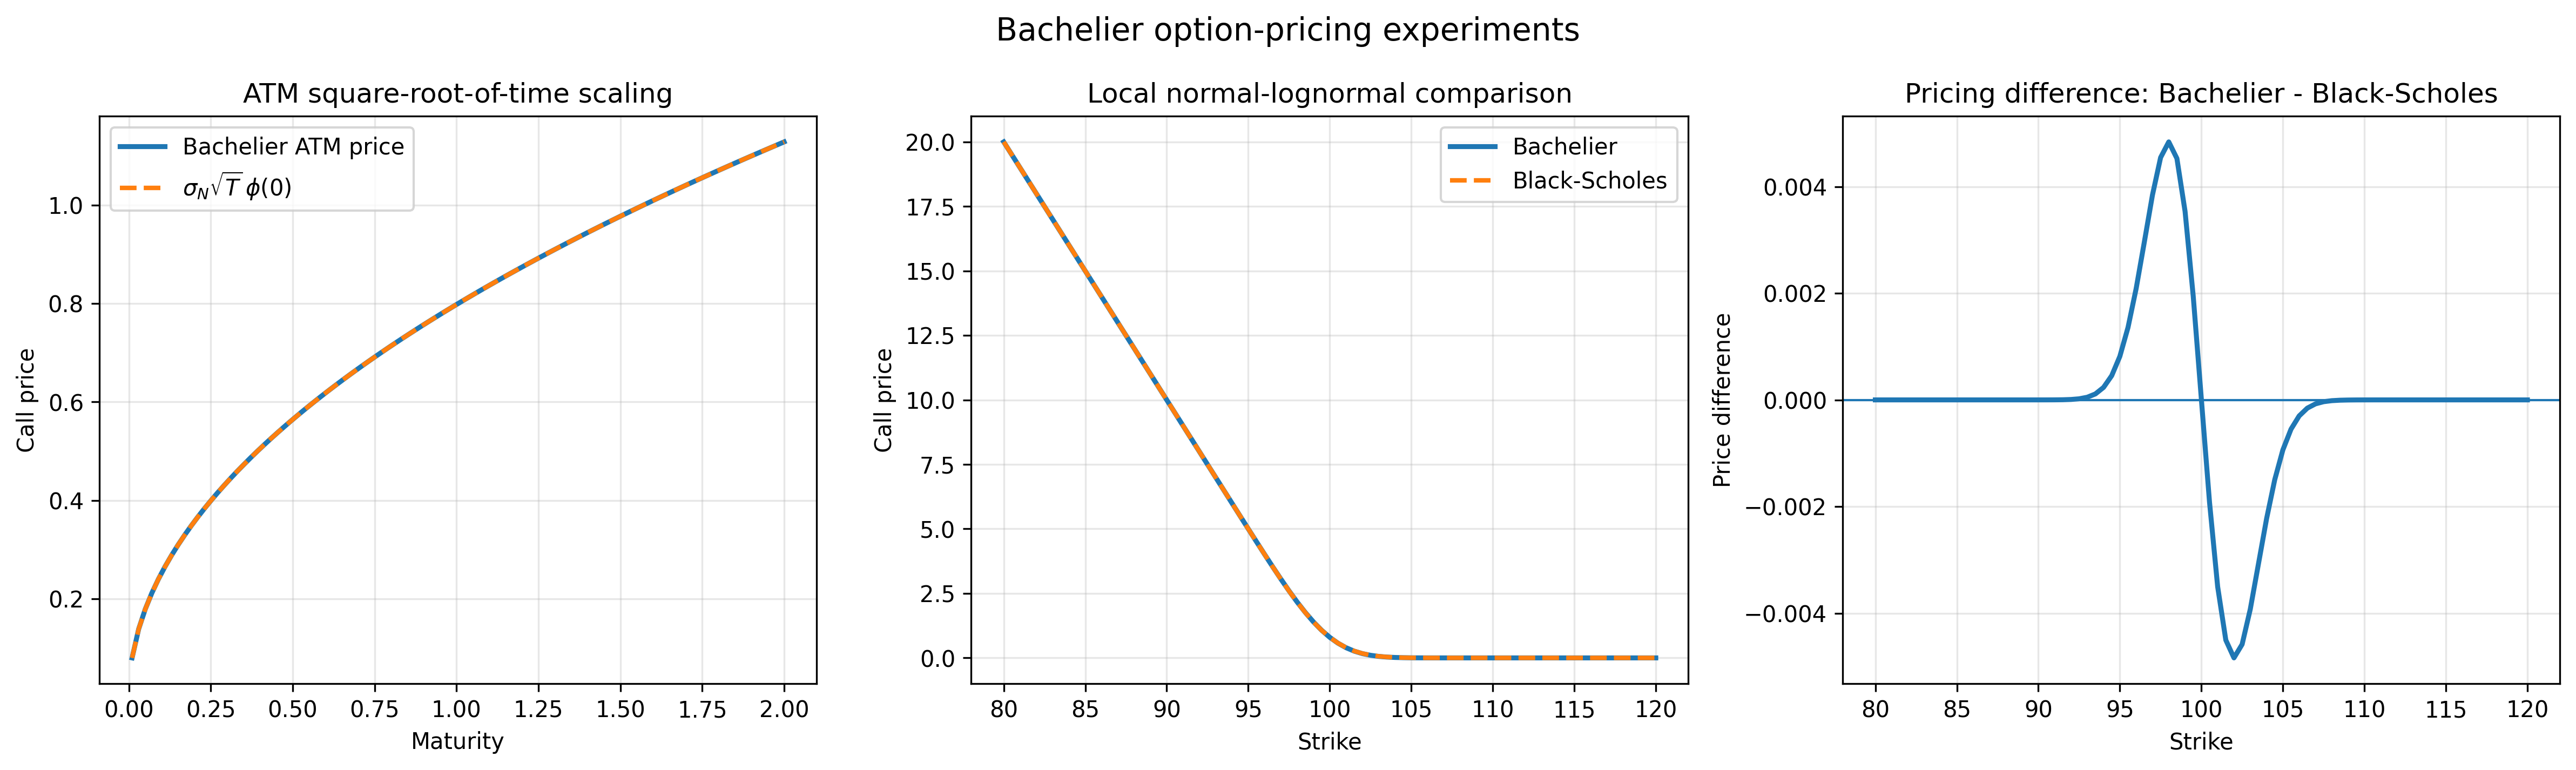
\includegraphics[width=\textwidth]{fig2_option_pricing_revised.png}
\caption{Normal option-pricing experiments. The left panel shows at-the-money square-root-of-time scaling. The centre panel compares normal and Black--Scholes prices under the local matching \(\sigma_N=S_0\sigma_{BS}\). The right panel displays the pricing difference, making visible a discrepancy that is nearly hidden when the two price curves are overlaid.}
\label{fig:option-pricing}
\end{figure}

% ==================================================================
\section{Local Comparison with Black--Scholes}
% ==================================================================

Under the Black--Scholes model,

\begin{equation}
\dd S_t=\mu S_t\dd t+\sigma_{BS}S_t\dd W_t.
\end{equation}

This specification models proportional changes and implies lognormal positive prices. The normal model instead describes absolute changes and permits negative values. The two architectures are not equivalent.

A first-order local comparison around \(S_0\) matches the diffusion coefficients through

\begin{equation}
\sigma_N\approx S_0\sigma_{BS}.
\label{eq:local-vol-matching}
\end{equation}

Equation~\eqref{eq:local-vol-matching} is a local, near-the-money, low-relative-volatility approximation. It is not a global transformation between normal and lognormal models.

For \(S_0=100\), \(\sigma_{BS}=0.02\), \(\sigma_N=2\), \(T=1\), zero rates, and strikes from \(80\) to \(120\), the maximum absolute price difference on the plotted grid is approximately

\begin{equation}
\max_K\left|C_{\mathrm{Bach}}(K)-C_{\mathrm{BS}}(K)\right|
\approx0.004839,
\end{equation}

attained near \(K=102\). The small absolute difference explains why the two curves are visually close in the centre panel of Figure~\ref{fig:option-pricing}; the difference panel shows that the models are nevertheless distinct.

Historically, Bachelier's model is not a failed Black--Scholes model. It is an earlier and structurally different normal modelling architecture. Modern normal-volatility applications, especially in rates, further demonstrate that the normal model can remain useful when its assumptions fit the instrument and market convention.

% ==================================================================
\section{Discussion}
% ==================================================================

The analytical and numerical results are mutually consistent. The simulated arithmetic process has an empirical mean close to the initial level, and its variance follows the predicted linear growth. The option experiment produces a Monte Carlo estimate whose discrepancy from the analytical normal price is negligible relative to sampling uncertainty.

The pricing section also makes explicit a distinction that is sometimes obscured in elementary presentations. Under a physical or statistical model, an expectation describes a forecast distribution. Under an arbitrage-pricing model, a discounted conditional expectation is taken under a pricing measure associated with a numeraire. The simple formula implemented in the code is valid as the zero-rate, unit-discount, forward-equals-initial-level special case of the more general normal forward formula.

From a historical perspective, Bachelier's achievement lies in introducing a probabilistic structure for speculation and contingent claims. Modern language---Brownian motion, filtrations, martingale measures, and numerical simulation---allows that achievement to be reconstructed without claiming that the later formalism appeared in its present form in 1900.

From an open-science perspective, the project treats a historical mathematical result as an executable research object: the model is stated, derived, coded, tested, visualized, versioned, and archived.

% ==================================================================
\section{Limitations}
% ==================================================================

The principal structural limitation of arithmetic Brownian motion is the possibility of negative prices. From equation~\eqref{eq:normal-price-distribution},

\begin{equation}
\Prob(P_t<0)=\Phi\!\left(-\frac{P_0}{\sigma\sqrt{t}}\right)>0
\end{equation}

for finite \(P_0>0\), \(\sigma>0\), and \(t>0\). In the baseline experiment, \(P_0/(\sigma\sqrt{T})=50\), so the probability is numerically negligible, but the theoretical issue remains.

The driftless process in Section~4 omits expected returns and is intentionally pedagogical. The pricing model in Section~5 similarly abstracts from stochastic rates, dividends, funding, transaction costs, liquidity, and market incompleteness. These elements matter in applications and should be incorporated when the instrument requires them.

Arithmetic Brownian motion also imposes symmetric Gaussian changes with constant normal volatility. Empirical financial series may exhibit skewness, heavy tails, volatility clustering, jumps, leverage effects, and regime changes \citep{mandelbrot1963,merton1976}. The model is therefore not a complete empirical description of markets.

The Black--Scholes comparison is deliberately local. Matching \(\sigma_N\) to \(S_0\sigma_{BS}\) does not produce global equivalence across large moneyness ranges, long maturities, nonzero rates, or changing volatility surfaces.

Finally, this reconstruction covers selected mathematical features rather than the full institutional, historical, and textual content of Bachelier's thesis. It should be read alongside the original source and specialist historical scholarship \citep{courtault2000,davisetheridge2006}.

% ==================================================================
\section{Reproducibility and Open-Science Framework}
% ==================================================================

The repository accompanying this paper includes source code, generated figures, fixed random seeds, automated tests, continuous-integration configuration, a reproduction notebook, citation metadata, authorship information, reproducibility documentation, and open-source licensing.

A successful reconstruction consists of four layers:

\begin{enumerate}[label=(\arabic*), leftmargin=2.2em]
\item the test suite completes successfully;
\item both numerical scripts execute from a clean environment;
\item the figures and reported tables are regenerated;
\item the paper compiles with resolved references and links.
\end{enumerate}

No external empirical dataset is used in this study. The numerical material consists of pseudo-random simulations generated from explicitly stated models, parameters, algorithms, and seeds.

The article is distributed under the Creative Commons Attribution 4.0 International licence. The accompanying software is distributed under the MIT License. These licences apply to different research objects and should not be conflated.

The concept DOI \ConceptDOI\ identifies the evolving Zenodo record and resolves to the latest published version. Each released paper version should also preserve its version-specific DOI in the Zenodo metadata and release notes.

% ==================================================================
\section{Conclusion}
% ==================================================================

Bachelier's \emph{Th\'eorie de la Sp\'eculation} remains foundational because it demonstrated that market fluctuations and contingent claims could be studied probabilistically. This paper has reconstructed a selected mathematical core using modern notation, a complete martingale argument, an explicit forward-measure pricing framework, fixed-seed numerical experiments, automated testing, and open research infrastructure.

The results reproduce the expected martingale and variance properties and numerically corroborate the normal call formula. The comparison with Black--Scholes clarifies that normal and lognormal models are locally close under a particular low-volatility matching, yet remain structurally distinct.

The project also illustrates a broader methodological principle: foundational quantitative-finance results can be made inspectable and executable. Historical scholarship, mathematical derivation, software engineering, uncertainty reporting, version control, and open archiving can be combined within a single reproducible research workflow.

% ==================================================================
\section*{Code and Research Materials Availability}
% ==================================================================

The code, tests, figures, notebook, LaTeX source, and reproducibility documentation are available at:

\begin{center}
\url{https://github.com/Alpha-Stochastic-Research/asr-theory-of-speculation}
\end{center}

No external empirical dataset was used. The article is licensed under CC BY 4.0; the software is licensed under the MIT License.

% ==================================================================
\section*{Declaration of Interest}
% ==================================================================

The author declares no competing financial interest related to this paper.

% ==================================================================
\section*{Acknowledgements}
% ==================================================================

The author acknowledges Louis Bachelier's historical contribution and the scholarship that has clarified the mathematical and institutional context of \emph{Th\'eorie de la Sp\'eculation}. This paper is part of the Alpha Stochastic Research programme for reproducible quantitative finance.

% ==================================================================
\appendix
\section{Reproduction Commands}
% ==================================================================

From the repository root:

\begin{verbatim}
git clone https://github.com/Alpha-Stochastic-Research/
    asr-theory-of-speculation.git
cd asr-theory-of-speculation

python -m venv .venv
source .venv/bin/activate

python -m pip install --upgrade pip
python -m pip install -e ".[dev]"

pytest -q
python src/brownian_motion.py
python src/option_pricing.py
\end{verbatim}

On Windows PowerShell, activate the environment with:

\begin{verbatim}
.venv\Scripts\Activate.ps1
\end{verbatim}

To compile the paper from the \texttt{paper/} directory:

\begin{verbatim}
pdflatex main.tex
bibtex main
pdflatex main.tex
pdflatex main.tex
\end{verbatim}

The figures are written to \texttt{figures/}. A pinned environment is recorded in \texttt{requirements-lock.txt}; the editable package configuration remains in \texttt{pyproject.toml}.

% ==================================================================
\section{Repository Structure}
% ==================================================================

\begin{verbatim}
asr-theory-of-speculation/
|-- .github/
|   `-- workflows/
|       |-- python-ci.yml
|       `-- publish-pypi.yml
|-- figures/
|   |-- fig1_random_walk_martingale.png
|   `-- fig2_option_pricing_revised.png
|-- notebooks/
|   `-- bachelier_theory_of_speculation_reproduction.ipynb
|-- paper/
|   |-- main.tex
|   |-- references.bib
|   `-- README.md
|-- src/
|   |-- asr/
|   |   `-- models/
|   |       `-- bachelier/
|   |           |-- __init__.py
|   |           |-- pricing.py
|   |           |-- process.py
|   |           `-- simulation.py
|   |-- brownian_motion.py
|   `-- option_pricing.py
|-- tests/
|   |-- conftest.py
|   |-- test_brownian_motion.py
|   |-- test_option_pricing.py
|   `-- test_package_imports.py
|-- AUTHORS.md
|-- CHANGELOG.md
|-- CITATION.cff
|-- LICENSE
|-- README.md
|-- REPRODUCIBILITY.md
|-- pyproject.toml
|-- requirements.txt
`-- requirements-lock.txt
\end{verbatim}

% ==================================================================
\bibliographystyle{plainnat}
\bibliography{references}

\end{document}
